\chapter{State of the Art}%
\label{chapter:State of the Art}

\begin{introduction}
This chapter will provide a comprehensive review of current \ac{5G} and Wi-Fi integration efforts, existing authentication mechanisms, and challenges in device identification. It will also explore recent developments and proposed solutions in the field, setting the context for our research.
\end{introduction}

\section{\acs{5G} Network Architecture}

\ac{5G} network represent a major shift from previous version in the sense that it is a \ac{SBA} which incorporates \ac{NFV} and \ac{SDN} technology. These changes allow for seperation between \ac{UP} and \ac{CP}, improving scalability, and flexibility of deployments, but most importantly, it allows for a unified authentication framework~\cite{23.501-p56}.

\subsection{Why \acs{4G} needed improved security?}

% !!! One of the problems is the USIM is expected ||
From the point of view of authentication, a cellular network consists of three main components: \acp{UE}, a \ac{SN}, and a \ac{HN}. Each \ac{UE} is expected to possesses a \ac{USIM} storing a cryptographic key, shared with the home network. In 4G networks, the serving network includes equipment like \acp{eNodeB} base stations, and  \acp{MMe} that manage connections. The \ac{UE} connects to this network through radio signals. The home network stores user information in a database called the \ac{HSS}, which handles authentication. Both networks communicate over an \ac{IP}-based system, and all the main components working together form the \ac{EPS}~\cite{cbl-comp-4g-5g-p3}.

In \ac{4G} \ac{EPS-AKA}, there are two significant flaws. First, during the initial stage of the authentication process, the \ac{UE} must transmit its identity, specifically its \ac{IMSI}, to the serving network. This identity is sent over the radio network without encryption, exposing it to potential interception~\cite{cbl-comp-4g-5g-p3}. Although a \ac{GUTI} may be used, researchers have demonstrated that \ac{GUTI} allocation is flawed in the sense that identifiers are not changes with enough frequency~\cite{gt-freq} or are allocated in a predictable pattern~\cite{gt-pred}. Second, during the authentication decision, the home network may provide an \ac{AV}, but this value is not directly included in the decision-making process, which is instead handled solely by the serving network~\cite{cbl-comp-4g-5g-p4}.

\begin{figure}[htbp]
    \centering
    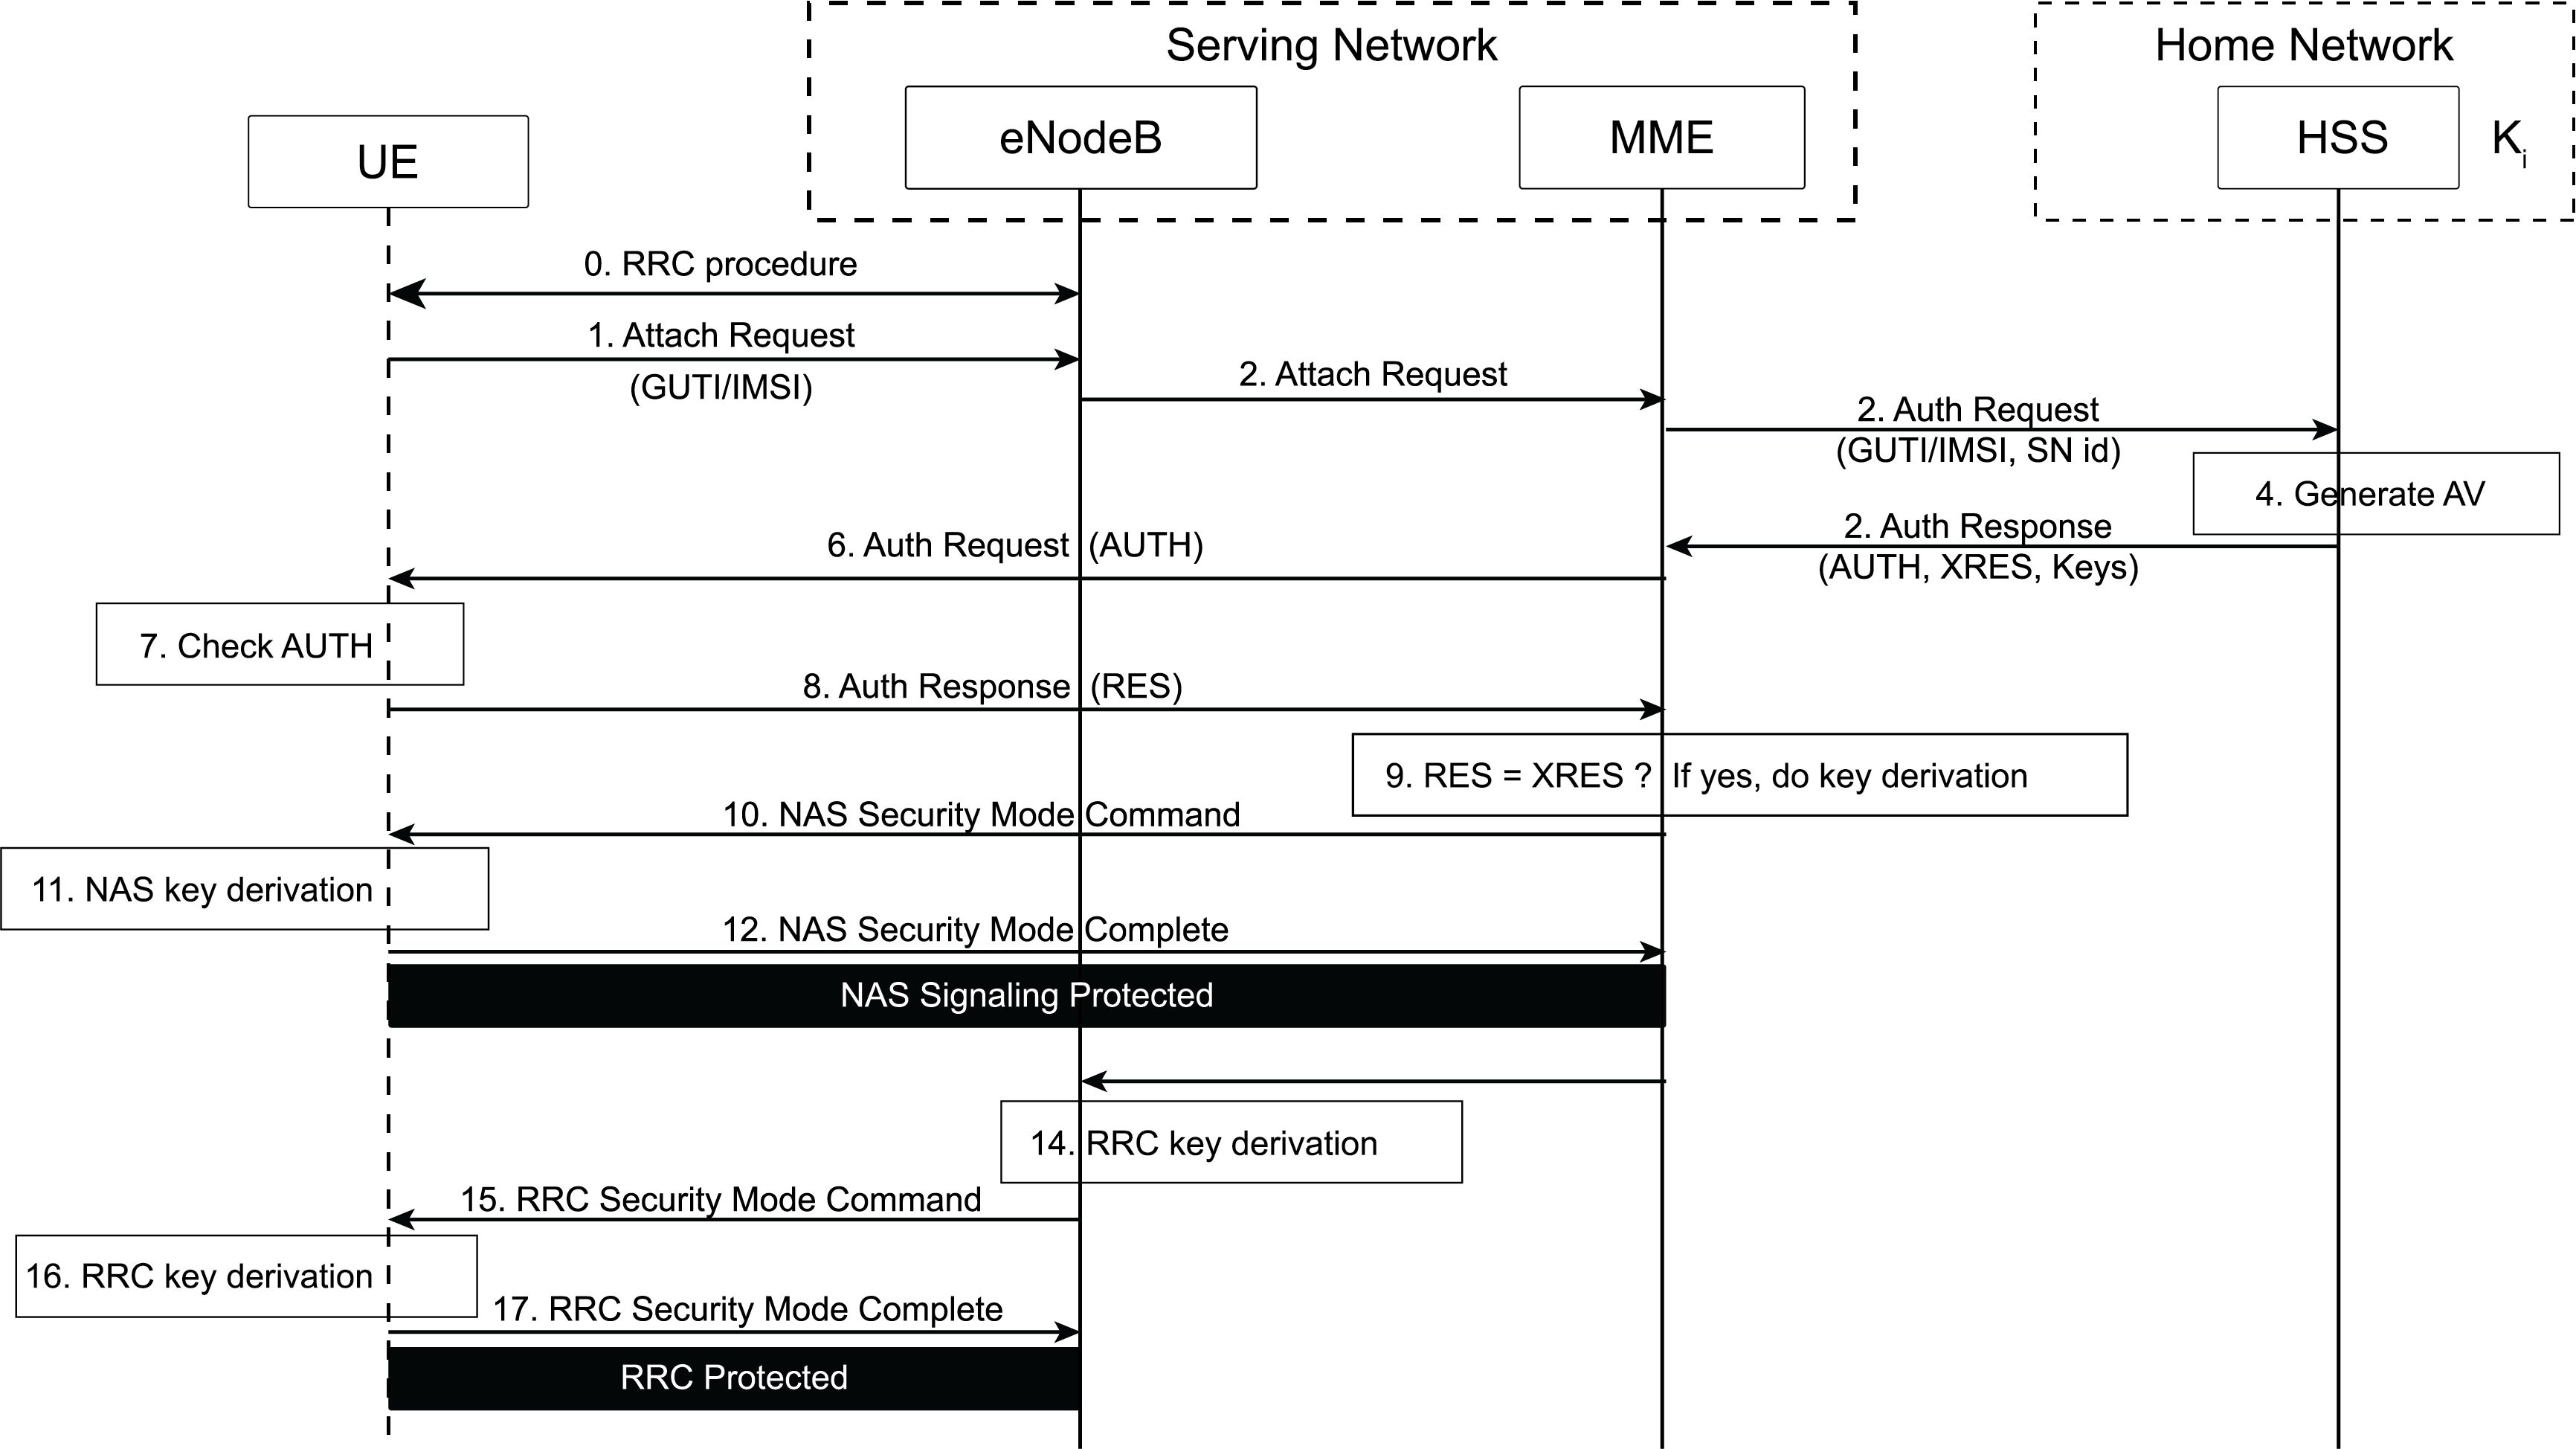
\includegraphics[width=0.8\textwidth]{figs/4g-authentication-flow.png}
    \caption{\ac{4G} Authentication Procedure}
    \label{fig:single}
\end{figure}

\subsection{\acs{5G} Security Framework}

As mentioned before, \ac{5G} has a \acl{SBA}, and in this architecture, some of the new entities relevant to \ac{5G} authentication are:

\begin{itemize}
    \item{
        The \ac{SEAF}, which acts as a intermidiary between the \ac{UE} and its home network, during the authentication process. It has the capability to out right reject and \ac{UE} but is dependent on the \ac{HN} to validate the authentication.
    }
    \item{
        The \ac{AUSF} is responsible to deciding if the \ac{UE} get authenticated.
    }
    \item{
        The \ac{UDM} hosts the \ac{ARPF}, responsible for selecting the authentication method, based on the subscribet identity and configured policy. It will also compute the authentication data for \ac{AUSF}.
    }
    \item{
        The \ac{SIDF} will be responsible for obtaining the \ac{SUPI} by decrypting the \ac{SUCI}.
    }
\end{itemize}

One of the main goals for \ac{5G} was the unification of authentication by making it open and access-network agnostic. In order to make it open, \ac{5G} rellies havily on \ac{EAP}, and when used the authentication will take place between the \ac{UE}, acting as the supplicant, the \ac{AUSF}, acting has the authenticaion server, through the \ac{SEAF} acting as an authenticator~\cite{rfc3748}.

Each generation of cellular networks has defined at least one new authentication method. For example, \ac{4G} introduced \ac{EPS-AKA}, and \ac{5G} introduced three authentication methods: \ac{5G-AKA}, \ac{EAP-AKA'}, and \ac{EAP-TLS}.

\subsection{Comparing \acs{5G-AKA}, \ac{EAP-AKA'} and \ac{EAP-TLS}}

The process begins when the \ac{SEAF} initiates authentication after receiving a message from the \ac{UE}. The \ac{UE} provides either a \ac{5G-GUTI} or a \ac{SUCI}.

The \ac{AUSF} first verifies that the requesting network is authorized. It then sends an authentication request to \ac{UDM}/\ac{ARPF}. If the \ac{SUCI} is provided, it's decrypted by the \ac{SIDF} to retrieve the \ac{SUPI}, which is then used to select the authentication method. \ac{UDM}/\ac{ARPF} generates an authentication response that includes tokens and keys, which are used by the \ac{AUSF} to compute a hash (\ac{HXRES}) and verify the expected response.

The \ac{AUSF} sends the authentication response to the \ac{SEAF} with the \ac{AUTH} token and \ac{HXRES}. At this point, the \ac{SUPI} is still not shared with the \ac{SEAF}. The \ac{SEAF} then forwards the \ac{AUTH} token to the \ac{UE}, which validates it using a secret key shared with the home network. If successful, the \ac{UE} computes and sends a response (\ac{RES} token) back to the \ac{SEAF}. The \ac{SEAF} validates this and forwards it to the \ac{AUSF} for final validation.

Once the \ac{RES} token is verified by the \ac{AUSF}, it sends an anchor key to the \ac{SEAF}, which then derives an \ac{AMF} key. The \ac{AMF} uses this key to generate further keys for protecting signaling messages between the \ac{UE} and the network elements. The \ac{UE}, with its root key, can derive all necessary keys for secure communication with the network, ensuring a shared and secure set of keys between the \ac{UE} and the network.

\ac{EAP-AKA'} is an alternative authentication method in \ac{5G}, providing mutual authentication between the \ac{UE} and the network based on a shared cryptographic key. Like \ac{5G-AKA}, it ensures strong security properties but has different message flows since it is based on \ac{EAP}. In this method, \ac{EAP} messages are encapsulated in \ac{NAS} messages between the \ac{UE} and the \ac{SEAF}, and in \ac{5G} service messages between the \ac{SEAF} and the \ac{AUSF}. In \ac{EAP-AKA'}, the \ac{SEAF} acts as a transparent relay, forwarding \ac{EAP} messages between the \ac{UE} and the \ac{AUSF} without participating in authentication decisions. In contrast, in \ac{5G-AKA}, the \ac{SEAF} verifies the \ac{UE}'s authentication response and can act on failures. Also, in 5G-AKA, the \ac{KAUSF} is computed by \ac{UDM}/\ac{ARPF} and sent to the \ac{AUSF} while in \ac{EAP-AKA'}, the \ac{AUSF} derives the \ac{KAUSF} from keying materials provided by the \ac{UDM}/\ac{ARPF}, using an \ac{EMSK} as specified in \ac{EAP}.

Lastly we have \ac{EAP-TLS} which is a subscriber authentication method in \ac{5G}, designed for specific scenarios like private networks and \ac{IoT}. When selected by \ac{UDM}/\ac{ARPF}, \ac{EAP-TLS} operates between the \ac{UE} and the \ac{AUSF} through the \ac{SEAF}, which acts as a transparent \ac{EAP} authenticator, forwarding \ac{EAP-TLS} messages. With \ac{EAP-TLS} we still achieve mutual authenticaion, this time via verification of public key certificates or a pre-shared key (\ac{PSK}) established through \ac{TLS} handshakes or out-of-band methods.

Some fundamental differences between this method and the previous AKA-based ones include the trust model: in \ac{EAP-TLS}, mutual trust is based on public key certificates, unlike AKA methods, which rely on symmetric keys shared between the \ac{UE} and the network. Additionally, \ac{EAP-TLS} eliminates the need to store numerous long-term symmetric keys in the home network (\ac{UDM}), reducing risks in key management. Another key difference that makes \ac{EAP-TLS} extremely well-suited for our use case is that it does not require the \ac{UE} to have a \ac{USIM}~\cite{cbl-comp-4g-5g-p12}.

\subsection{What is \ac{3GPP} and non-\ac{3GPP} access?}

ac{3GPP} encompasses standards for mobile networks like \ac{3G}, \ac{4G}, and \ac{5G}, which are cellular technologies enabling network services from mobile carriers. In contrast, non-\ac{3GPP} refers to access technologies not standardized by \ac{3GPP}, such as Wi-Fi or satellite networks, which can still integrate with \ac{3GPP} networks but follow different standards (e.g., IEEE for Wi-Fi).

Within \ac{3GPP} architecture, the terms trusted and untrusted define how non-\ac{3GPP} networks connect to the mobile core. Trusted networks are verified and approved by the mobile operator, connecting directly to the core network using secure protocols, similar to \ac{3GPP} networks. For instance, a mobile operator’s managed Wi-Fi network may be trusted. On the other hand, untrusted networks, like public Wi-Fi hotspots managed by third parties, do not meet these standards and are treated differently.

\section{Wi-Fi Integration Challenges}

\section{Authentication and Identity Management in \acs{5G}}

% subsection:
%   - What is a GUTI, SUPI, SUCI and NAI?

\section{Current Solutions and Proposals}